\documentclass[11pt,letterpaper]{article}
\pdfinfoomitdate=1\pdftrailerid{}\pdfsuppressptexinfo=15
\usepackage[T1]{fontenc}\usepackage[utf8]{inputenc}
\usepackage{lmodern,mathpazo,microtype}
\usepackage[margin=.87in,headheight=15pt]{geometry}
\usepackage{amsmath,amssymb,amsthm,mathtools}
\usepackage{graphicx,xcolor,booktabs,tabularx,array,longtable,enumitem,tikz}
\usetikzlibrary{arrows.meta,positioning,calc,fit}
\usepackage{titlesec,fancyhdr,needspace,placeins,listings,xurl}
\usepackage[numbers,sort&compress]{natbib}
\usepackage[colorlinks=true,linkcolor=violetink,citecolor=violetink,urlcolor=tealink,bookmarksnumbered]{hyperref}
\definecolor{ink}{HTML}{241B38}\definecolor{violetink}{HTML}{674499}
\definecolor{tealink}{HTML}{126E70}\definecolor{gold}{HTML}{A7803C}
\definecolor{pale}{HTML}{F5F2FA}\definecolor{muted}{HTML}{655E72}
\definecolor{brightgold}{HTML}{EBC577}\definecolor{brightteal}{HTML}{9EDCD1}
\hypersetup{pdftitle={AGI ALPHA FLYWHEEL 2026 11 02 Report},pdfauthor={Vincent Boucher},pdfsubject={Constructing the means of consequential progress: source-bound experiments and economic continuation}}
\urlstyle{same}\setlength{\emergencystretch}{3em}
\setlength{\parindent}{0pt}\setlength{\parskip}{5pt}\linespread{1.025}
\newcolumntype{Y}{>{\raggedright\arraybackslash}X}
\newcolumntype{P}[1]{>{\raggedright\arraybackslash}p{#1}}
\newcommand{\OmegaH}{SUCCESSOR~$\Omega$}
\newcommand{\repo}{https://github.com/MontrealAI/AGI-Alpha-Invention-Flywheel-Lab}
\newcommand{\lead}[1]{\Needspace{5\baselineskip}\par\medskip\noindent{\large\bfseries\color{violetink}#1}\par\smallskip}
\newcommand{\insight}[1]{\begin{center}\setlength{\fboxsep}{9pt}\fcolorbox{violetink}{pale}{\begin{minipage}{.94\linewidth}#1\end{minipage}}\end{center}}
\newtheorem{proposition}{Proposition}\newtheorem{definition}{Definition}
\setlist{leftmargin=1.3em,itemsep=2pt,topsep=4pt}
\renewcommand{\arraystretch}{1.15}\setlength{\tabcolsep}{5pt}
\titleformat{\section}{\large\sffamily\bfseries\color{ink}}{\color{violetink}\thesection}{.6em}{}
\titleformat{\subsection}{\normalsize\sffamily\bfseries\color{ink}}{\thesubsection}{.6em}{}
\titlespacing*{\section}{0pt}{17pt}{7pt}\titlespacing*{\subsection}{0pt}{11pt}{5pt}
\pagestyle{fancy}\fancyhf{}\fancyhead[L]{\footnotesize\sffamily AGI ALPHA FLYWHEEL}
\fancyhead[R]{\footnotesize\sffamily 2026 11 02 REPORT}\fancyfoot[L]{\scriptsize\sffamily MONTREAL.AI / QUEBEC.AI}
\fancyfoot[R]{\small\color{violetink}\thepage}\renewcommand{\headrulewidth}{.3pt}
\lstset{basicstyle=\footnotesize\ttfamily,columns=fullflexible,breaklines=true,keepspaces=true,frame=single,rulecolor=\color{violetink!35},showstringspaces=false}
\renewcommand{\topfraction}{.95}\renewcommand{\bottomfraction}{.9}\renewcommand{\textfraction}{.05}\renewcommand{\floatpagefraction}{.8}
\begin{document}
\begin{titlepage}\pagecolor{ink}\color{white}\thispagestyle{empty}

\begin{tikzpicture}[remember picture,overlay]
\fill[violetink!45!ink] ([xshift=-1cm,yshift=-1cm]current page.north east) circle (5cm);
\foreach \r in {3.1,3.5,3.9,4.3,4.7}{\draw[white,opacity=.065] ([xshift=-1cm,yshift=-1cm]current page.north east) circle (\r cm);}
\draw[brightgold,line width=1.8pt] ([xshift=2.2cm,yshift=2.7cm]current page.south west)--([xshift=19.2cm,yshift=2.7cm]current page.south west);
\end{tikzpicture}
{\sffamily\small MONTREAL.AI / QUEBEC.AI\hfill\color{brightgold}RESEARCH REPORT}\par
\vspace{17mm}
{\sffamily\bfseries\fontsize{18}{23}\selectfont AGI ALPHA}\par\vspace{2mm}
{\sffamily\bfseries\fontsize{47}{51}\selectfont FLYWHEEL}\par\vspace{6mm}
{\sffamily\fontsize{24}{29}\selectfont 2026 11 02 Report}\par\vspace{8mm}
{\sffamily\fontsize{20}{26}\selectfont Constructing the means\\of consequential progress.}\par\vspace{9mm}
{\sffamily\color{brightteal}TRANSFORMATIONAL INTELLIGENCE $\boldsymbol{\infty}$}\par
\vspace{12mm}
\begin{center}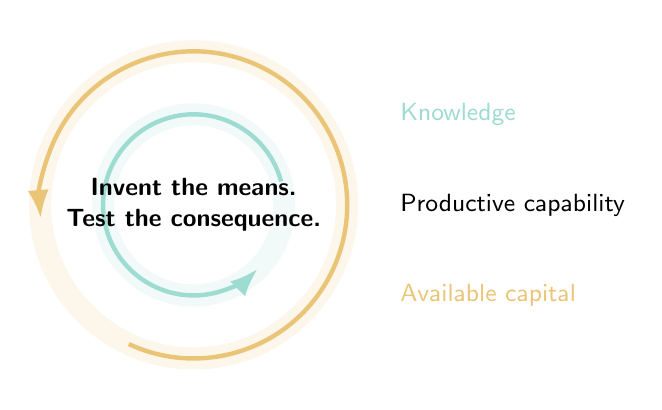
\begin{tikzpicture}[>=Latex]
\foreach \r/\c/\a in {1.15/brightteal/15,1.55/white/130,1.95/brightgold/245}{\draw[\c,opacity=.15,line width=8pt] (0,0) circle (\r);\draw[\c,line width=1.6pt,->] (\a:\r) arc[start angle=\a,end angle=\a+300,radius=\r];}
\node[align=center,font=\sffamily\bfseries\small] at (0,0) {Invent the means.\\Test the consequence.};
\node[anchor=west,font=\sffamily\small,brightteal] at (2.5,1.15) {Knowledge};
\node[anchor=west,font=\sffamily\small] at (2.5,0) {Productive capability};
\node[anchor=west,font=\sffamily\small,brightgold] at (2.5,-1.15) {Available capital};
\end{tikzpicture}\end{center}
\vfill
{\large\bfseries Vincent Boucher}\par\smallskip
MONTREAL.AI\quad\textbullet\quad QUEBEC.AI\par
Montr\'eal, Qu\'ebec, Canada\par\medskip
{\small\color{white!75}Research period: 2 November 2026\par
Source and publication review: 3 November 2026\par
Report edition 1.0\quad\textbullet\quad Public evidence, explicit scope}
\vspace*{15mm}
\end{titlepage}\nopagecolor\color{ink}

\lead{Build the missing means. Establish what they make possible.}
\begin{abstract}
An invention flywheel becomes consequential when a verified construction changes what a successor can observe, produce, accept or afford. This report examines that proposition through source-bound AGI ALPHA experiments associated with 2 November 2026. It connects typed program construction, metrology, purpose-preserving decisions, complementary production, discovery allocation, operating benchmarks and native financial simulations without conflating their evidence. A three-generation foundry constructs 30 accepted programs and six nonidentifiability certificates per arm; accumulation reduces arithmetic relative to weaker retention but the conventional compiler is substantially cheaper. A paired-acquisition instrument passes 80 material and 12 spatial model cases while preserving four undetected-error witnesses and conventional ties. Manufacturing witnesses show why accurate average measurements need not identify local stress. A measured biological-panel replay finds 14 targets in 23 queries, compared with 15 for strong conventional controls. Separately, 110 native authored financial accounts complete their registered horizons: the best final trailing-year profit is zero, 23 retain uncovered obligations, and actual revenue remains zero. A different seven-account experiment demonstrates conditional earned-funded resource continuation, with no retained-method advantage and seed-backed collateral. We reproduce selected computational checks and provide a compact arithmetic auditor and complete result denominators. The contribution is an operational synthesis and decision-relevant evidence map: construct the enabling means, establish fresh acceptance, compare complete alternatives and finance continuation from valid available resources. Large-scale scientific production and sustained commercial compounding remain objectives, with specific next tests rather than inferred achievements.
\end{abstract}

\insight{\textbf{The question is a construction problem.}\par\smallskip
Which valuable outcome remains unavailable because something necessary cannot yet be measured, built, coordinated, verified or afforded---and what concrete means could remove that constraint?}

\textbf{How to read.} Sections~1--3 set out the mechanism and evidence rules. Sections~4--8 examine actual constructions and their controls. Sections~9--11 connect them to economic and physical expansion. The appendix gives exact source pins, replay scope and publication instructions. This is a synthesis of separately identified studies, not one pooled experiment or enterprise. The original research editions and result identities remain available.

\textbf{Evidence boundary.} Research edition dated 2 November; source-status review on 3 November. Main source snapshot: \nolinkurl{215b22a5ed73b82ac1d909328d60157c48bd9958}. Open-branch studies keep their separate exact revisions. Later Enterprise078 repairs are separated from the period's experiments. Original scientific protocols vary in exposure and registration timing; their claims are not upgraded by this report. Author-supplied editorial context informs the research questions; only public sources and original report prose are published.

\clearpage
\section{The next starting point}
A manufacturing decision can fail even when the fitted measurements look excellent. If two admissible stress fields produce the same observations but require different release decisions, a larger fit cannot identify which part is acceptable. The useful construction is an observation or decision method that removes the actual ambiguity. If the beneficiary needs a stress difference already identified by the measurements, a new purpose-preserving interface may suffice. If the beneficiary needs absolute local stress, a new calibrated observation may be necessary.

This is a concrete version of the AGI ALPHA ambition: construct means that make important work newly attainable, then use the qualified means to support a different useful construction. The productive asset may be an instrument, a representation with a valid decoder, a verified production boundary, an experimental interface or a voluntary arrangement that finances qualification. Its value is the consequence it can establish for the next task. The number of agents, artifacts or steps is not that consequence.

Library learning and executable abstractions have primary precedents in DreamCoder; archive-based agent self-modification is studied in the Darwin G{\"o}del Machine \cite{dreamcoder,dgm}. Those systems are not evaluated or outperformed here. The project has built and tested several parts of this mechanism. Programs execute and produce inspectable outputs. Controls expose failed transfer. Financial histories distinguish collected revenue from hypothetical capital. Some mathematical instruments identify precisely what a proposed application cannot infer. These are useful achievements at their stated scope. They neither establish a generally superintelligent organization nor demonstrate the market, industrial capacity or retained profit needed for very large expansion.

\subsection{A useful architecture must admit a better ordinary method}
Transformational Intelligence makes the formulation itself an object of construction: representations, observations, assumptions, coordination rules and intermediate requirements may change while the authorized purpose remains the reference \cite{ti}. Conventional mathematics and engineering are legitimate components. A familiar method can be the right enabling construction. A new architecture does not receive credit merely for renaming it.

The strongest comparison gives a competent conventional alternative the same observations, permitted actions, construction budget, rights and financing opportunities. It may construct its own tools or use the same retained content. Several experiments reviewed here show exactly such ties. The instrument-foundry's ordinary rank-aware compiler wins its complete arithmetic comparison. These findings favor adoption of the stronger method and narrow the new claim; they do not make the useful artifact disappear.

The report's scientific contribution is an evidence-linked synthesis, not a new sweep, inverse solver, linear program or general discovery algorithm. It identifies which connection between construction and consequence has actually been tested and which next test could change a decision. That makes it an implementation and investment document as well as a research report.

\section{Two flywheels, separately earned}
AGI ALPHA is the organizational substrate for agents, tools, work, evidence and retained capability \cite{foundation}. The commercial loop seeks a complete accepted outcome, voluntary purchase, collection, covered obligations and sustainable continuation. It can operate with fixed AI capabilities. The invention loop seeks new productive means and tests whether those means improve a fresh successor. Improvement in the procedure that discovers those means is a further claim.

\begin{figure}[htbp]\centering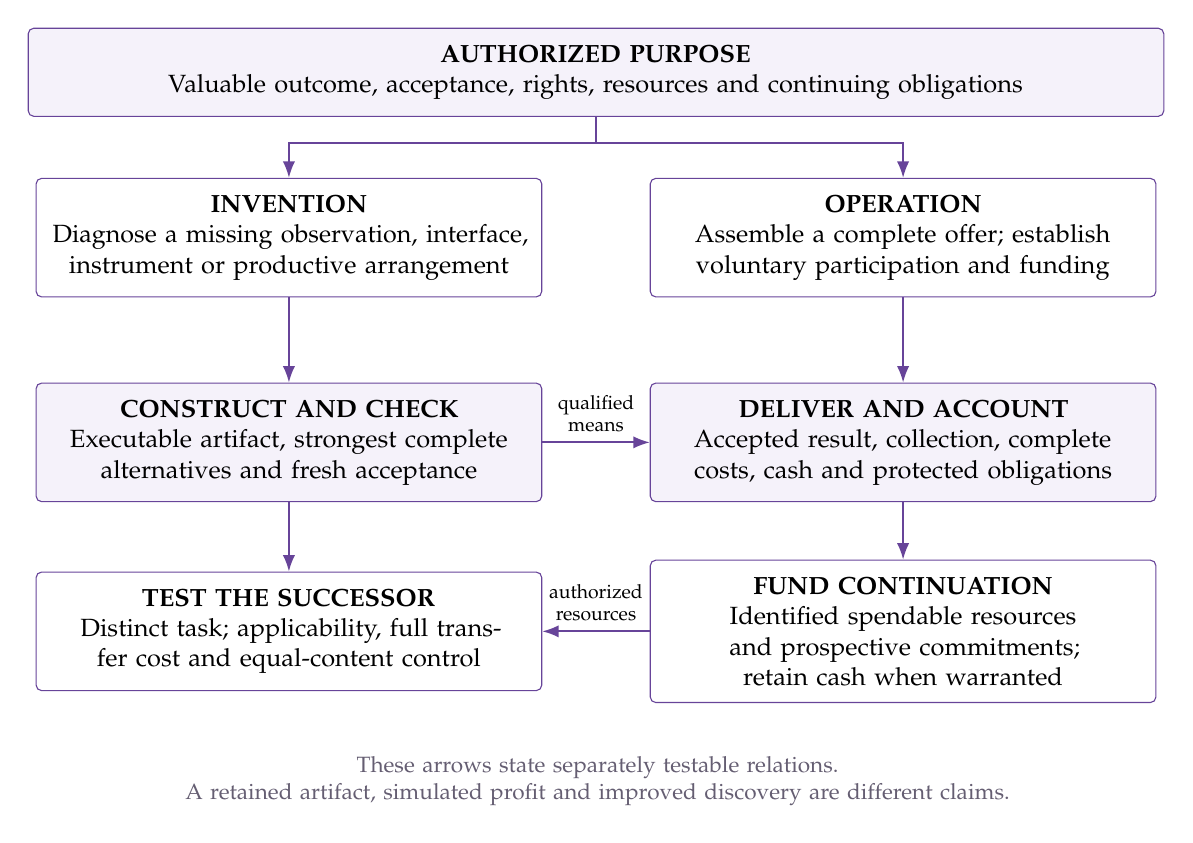
\begin{tikzpicture}[font=\small,>=Latex,b/.style={draw=violetink,rounded corners=2pt,align=center,inner sep=6pt},a/.style={->,draw=violetink,line width=.65pt}]
\node[b,fill=pale,text width=14cm] (purpose) at (0,0) {\textbf{AUTHORIZED PURPOSE}\par Valuable outcome, acceptance, rights, resources and continuing obligations};
\node[b,text width=6cm] (i1) at (-3.9,-2.1) {\textbf{INVENTION}\par Diagnose a missing observation, interface, instrument or productive arrangement};
\node[b,text width=6cm] (o1) at (3.9,-2.1) {\textbf{OPERATION}\par Assemble a complete offer; establish voluntary participation and funding};
\draw[a] (purpose.south)--(0,-.9)-|(i1.north);\draw[a] (purpose.south)--(0,-.9)-|(o1.north);
\node[b,fill=pale,text width=6cm] (i2) at (-3.9,-4.7) {\textbf{CONSTRUCT AND CHECK}\par Executable artifact, strongest complete alternatives and fresh acceptance};
\node[b,fill=pale,text width=6cm] (o2) at (3.9,-4.7) {\textbf{DELIVER AND ACCOUNT}\par Accepted result, collection, complete costs, cash and protected obligations};
\draw[a] (i1)--(i2);\draw[a] (o1)--(o2);
\draw[a] (i2.east)--node[above,font=\scriptsize,align=center]{qualified\\means}(o2.west);
\node[b,text width=6cm] (i3) at (-3.9,-7.1) {\textbf{TEST THE SUCCESSOR}\par Distinct task; applicability, full transfer cost and equal-content control};
\node[b,text width=6cm] (o3) at (3.9,-7.1) {\textbf{FUND CONTINUATION}\par Identified spendable resources and prospective commitments; retain cash when warranted};
\draw[a] (i2)--(i3);\draw[a] (o2)--(o3);
\draw[a] (o3.west)--node[above,font=\scriptsize,align=center]{authorized\\resources}(i3.east);
\node[align=center,text width=14cm,font=\footnotesize\color{muted}] at (0,-9) {These arrows state separately testable relations.\par A retained artifact, simulated profit and improved discovery are different claims.};
\end{tikzpicture}

\caption{Two coupled operating relations. Qualified capability may support production; genuinely available resources may fund construction. Each arrow requires its own evidence, cost and authority. The report supplies partial computational and simulated instances, not a fully validated self-expanding industrial system.}\label{fig:architecture}
\end{figure}

Four relation labels keep the architecture inspectable. \textbf{Reused by} means a fresh task actually invokes a retained artifact. \textbf{Constructed with} means inherited means participate in creating a different artifact, with an intervention testing their contribution. \textbf{Financed by} names the resources that paid for commitments, distinguishing initial equity, collected earnings and other financing. \textbf{Discovered better by} requires a changed discovery procedure to outperform a frozen and strong alternative on fresh campaigns at matched complete resources.

These relations do not imply each other. A program may reuse another without being cheaper. A profitable operation may involve no invention. An accepted invention may have no willing buyer. A useful retained library may improve task execution while leaving discovery unchanged. Authority, money, consent and legal rights never transfer merely because code or a parent identifier transfers.

The practical responsibilities remain OUT-LEARN, OUT-THINK, OUT-DESIGN, OUT-STRATEGISE, OUT-EXECUTE and OUT-EVOLVE \cite{outlearn,outthink,outdesign,outstrategise,outexecute,outevolve}. They are available methods rather than six mandatory model calls. Observation and calibration support learning; representations support reasoning; instruments and production boundaries support design; information and actions are chosen jointly; valid progress is retained during execution; fresh successors test what can be inherited. OUT-REFLECT concerns checkable evidence, and OUT-ACCELERATE asks whether the complete path to an accepted result becomes faster after acquisition and verification costs \cite{outreflect,outaccelerate}.

\FloatBarrier
\section{What was reviewed and what was rerun}
The report uses public source revisions for the two five-route portfolios, optical/water work, paired acquisition, manufacturing identifiability, NEXT072, two distinct outlearning streams, grid074, operational075 and the published foundry. These are selected consequential constructions associated with the research period; this is not an exhaustive audit of every historical campaign in the repository. Original identifiers distinguish similarly named routes. In particular, the 110-account public portfolio and the separate 24-arm portfolio are not combined.

The compact source map records 18 public files with commit, Git blob and SHA-256 identities. Numeric observations retain complete denominators for the claims extracted. No raw private account authority, user source document, internal conversation or large external dataset is republished. A pinned public link supports provenance; an internally coherent receipt does not establish external truth.

\begin{table}[htbp]\centering\small
\begin{tabularx}{\linewidth}{@{}P{3.0cm}YY@{}}\toprule
Evidence class & Report use & Boundary\\\midrule
Executed reproduction & Foundry replay; paired acquisition; separate N1 and N3 verifier programs & Same exposed inputs and source; no fresh physical or market sample\\
Compact recalculation & 110 R2 case summaries, exact money identities, control counts and report witness & Not a full independent replay of 110 signed native histories\\
Source-reviewed result & Other public study reports and their recorded independent verdicts & New publication does not turn their reports into a new experiment\\
Proved illustration & Linear identifiability condition and exact null-direction example & Declared linear model, no physical instrument qualification\\
Proposed next test & Scope-matched physical observations, complete offers and fresh successor comparisons & Not yet executed, funded or accepted\\\bottomrule
\end{tabularx}
\caption{Different evidence roles remain separate. ``Independent'' in original studies generally means procedural separation on a shared host, not external institutional certification.}\label{tab:classes}
\end{table}

The foundry replay compares all scientific fields, excluding only recorded Python-version metadata and observational timings. The paired run verifies its frozen source before and after execution. N1's independent verifier reproduces 18 expected outcomes; N3's reproduces 26. This report's independent arithmetic path checks all 110 compact case identities, profit/cash/payable relations, milestone flags and control denominators. It does not claim to recover omitted native raw exports or authenticate private record preimages. Seven mutation tests include lost losses, removed obligations, missing cases and equity relabeled as profit.

Historical preregistration is reported accurately. Some protocols were publicly committed before outcomes; the public portfolio's scientific protocols were local commits before outcomes and publicly published later. Public, authored cases are not protected holdouts. Multiple controls sharing the same observations are not independent market or biological replications. Previously failed source closures, interrupted runs, changed tolerances and supplemental controls retain their original status.

\section{Constructing the next instrument}
The published flywheel edition 1.1 makes one small construction mechanism executable \cite{flywheel11}. A typed program constructor receives observations, a target quantity, permitted primitives and eligible retained programs. It builds an expression, supplies a coefficient certificate, and evaluates it on fresh latent inputs. A successor can call an earlier accepted program on the current measurements. The actual retained object is executable code with identity and applicability conditions, rather than a saved answer.

Twelve authored episodes contain three requests each, compared under four arms: fresh construction, a frozen first-generation library, accumulating inheritance and a conventional rank-aware compiler. The same 36 requests per arm cover shared substructure, disjoint targets, changed identities and rank deficiency. Every arm accepts 30 programs and produces six certified nonidentifiability results; seven separate invalidation and exhaustion controls pass. The 144 request records are a crossed finite comparison, not 144 inventions or enterprises.

\begin{table}[htbp]\centering\small
\begin{tabularx}{\linewidth}{@{}Yrrr@{}}\toprule
Arm & Accepted / requests & Nonidentifiable & Scalar arithmetic\\\midrule
Fresh construction & 30/36 & 6 & 51,633\\
First-generation retention & 30/36 & 6 & 49,041\\
Accumulating retention & 30/36 & 6 & 48,141\\
Conventional rank-aware reuse & 30/36 & 6 & \textbf{13,566}\\\bottomrule
\end{tabularx}
\caption{Recorded finite construction study, exactly replayed for this report. Arithmetic includes construction, checking and execution in its declared counter; it is not money, energy or complete developer effort.}\label{tab:foundry}
\end{table}

One shared-structure lineage is $p_1(y)=y_0+y_1$, $p_2(y)=p_1(y)+y_2$, $p_3(y)=p_2(y)+y_3$. Calls execute on the current input and expand to their actual arithmetic cost. The accumulating and conventional arms produce the same typed lineage. This establishes constructive succession within the supplied language. It does not show the compiler learning a better discovery policy.

Accumulation saves 900 operations against first-generation-only retention in aggregate. It helps shared structure, adds archive/search work for disjoint targets, and does not reduce execution arithmetic: all arms use 141 execution operations. The conventional method is cheaper in every family. Retain its construction while keeping the other arms as explanatory controls. More retained content is not uniformly better.

\begin{figure}[htbp]\centering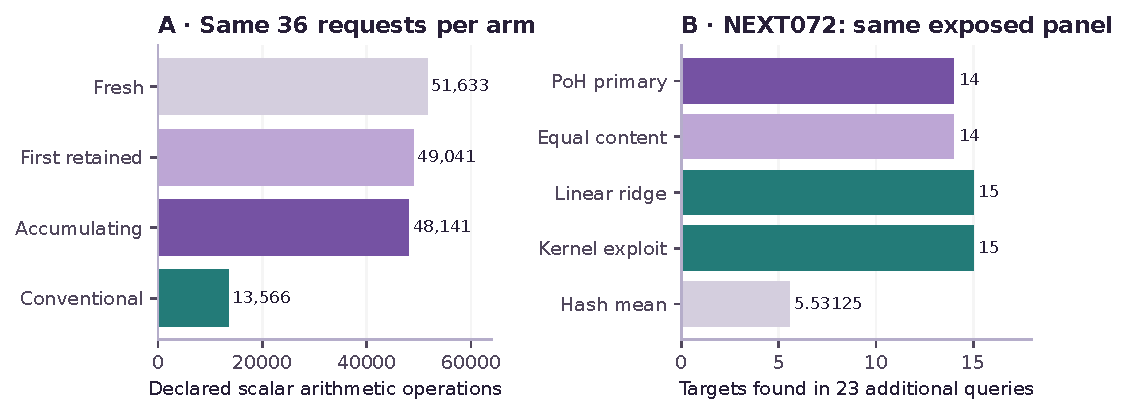
\includegraphics[width=\linewidth]{figures/comparators.pdf}
\caption{Strong complete controls change interpretation. A: all four foundry arms face the same requests and acceptance; conventional compilation is cheapest. B: NEXT072's primary passes its registered threshold but conventional predictors find one more target on the same exposed panel. Different panels and units are not pooled.}\label{fig:comparators}
\end{figure}

The distinction between continuation and complete-policy reachability also matters. If an initial comparator may construct and use the same tool under the same total budget, that entire sequence is already one of its available policies. A built tool can improve the current state or reduce a bounded search burden without expanding the union of all complete initial policies. A new frontier claim must specify the original restriction, the complete competitor and the actual cost of removing it \cite{flywheel11,ti}. This is how useful engineering remains creditable without manufacturing an unrestricted impossibility claim.

\section{Observation is a productive capability}
\subsection{Optical lineage: a real model construction, an unbuilt instrument}
The I1 study constructs a reciprocal optical inverse method with a distinct successor function \cite{i1}. Two designed-reflector responses support maximum attainable target intensity; a third coupled reflector resolves relative signs needed for coherent field reconstruction. Twenty-seven noiseless cases pass within 189 finite cases, and a separately generated ideal replay also passes 27/27. Noisy returns are not promises of physical accuracy.

The complete probe lineage costs $3n$ columns: $2n$ for K1 and $n$ more for K2. Fresh ordinary construction also costs $3n$ and matches the result. A wrong reflector amplitude can produce approximately 9.09\% field bias despite a tiny residual, and stale calibration can fail badly. The missing productive means is a realizable calibrated reflector arrangement with the required geometry and access, rather than a more impressive ideal-matrix fit. No physical optical commissioning, commercial acceptance or profit is established.

\subsection{Paired acquisition: remove a nuisance by changing the experiment}
The paired-acquisition follow-up supplies an especially clear transformational mechanism \cite{paired}. It exchanges specimen and blank paths between frames. Under its declared model, let corrected readings be
\[
a_0=g_A f_0 s,\quad b_0=g_B f_0,\qquad
a_1=g_A f_1,\quad b_1=g_B f_1 s,
\]
where $s$ is specimen transmission, $g_A,g_B$ are fixed path gains and $f_0,f_1$ are shared frame fluxes. Then
\begin{equation}
\frac{1}{2}\log\!\left(\frac{a_0/b_0}{a_1/b_1}\right)=\log s.
\end{equation}
The exchanged acquisition changes the available sufficient measurement. Fixed unequal gains and shared flux cancel algebraically; independent physical assumptions about dark correction, drift, blank validity, spectrum and geometry still require qualification.

The registered model contract passes 80/80 material cases, 12/12 spatial fields and eight scope/invalid-input controls. Eight well-separated fields complete all cell decisions; four boundary fields appropriately abstain on uncertain cells. All four registered undetected-error witnesses remain reproduced. An ordinary same-observation solver and fresh equal-content construction tie. Independent blank calibration also meets the finite decision standard and can use one specimen exposure, whereas paired acquisition requires two. Equal signal-error assumptions do not establish equal photons, dose, elapsed time or cost.

This report reproduces the frozen numerical run successfully. Its result is a model-valid acquisition instrument and explicit limits, not measured physical exposures or industrial savings. Six read-only capital/exposure projections retain HOLD or REFUSE; no native financial account, sale or financing receipt was created. The construction removes one nuisance dependence under assumptions, not every condition needed for an enterprise.

\subsection{Manufacturing: construct the observation the decision actually needs}
N3 provides a useful bridge between instrument design and qualification \cite{nextseries}. In a declared local isotropic linear-elastic model, a directional strain is
\begin{equation}
e_q=\big((1+\nu)q^\top\sigma q-\nu\operatorname{tr}\sigma\big)/E.
\end{equation}
For $E=200{,}000$ MPa and $\nu=0.3$, exact X/Z observations identify $\sigma_{xx}-\sigma_{zz}$ but not generally $\sigma_{xx}$. Tilted directions and unknown shears can destroy that simpler invariant. Material law, spatial kernel, direction and intended target must therefore be part of the instrument's interface.

\begin{proposition}[Linear observation sufficiency]
With unrestricted $x\in\mathbb R^n$, exact observations $y=Hx$ identify the scalar target $q^\top x$ for every $x$ if and only if $q$ lies in the row space of $H$. If $Hv=0$ and $q^\top v\ne0$, no deterministic estimator using only $y$ can be correct on both $x$ and $x+v$.
\end{proposition}
\begin{proof}
If $q=H^\top a$, the target is $a^\top y$. Otherwise the row-space/nullspace orthogonality relation supplies $v\in\ker H$ with $q^\top v\ne0$; the same observation has different required answers. The stated impossibility follows. Additional state restrictions, noise or approximate targets require their own contracts.
\end{proof}

The report's exact rational illustration uses the normal-stress direction $v=(1,7/3,1)$. Both X/Z strain changes are zero, while $\sigma_{xx}$ changes by one and $\sigma_{xx}-\sigma_{zz}$ remains unchanged. The companion checks this identity independently with fractions. It is an explanatory calculation, not another physical sample or a new linear-algebra theorem.

N3 also constructs mechanically admissible authored fields whose center stresses are $-100$ and $+100$ MPa while their declared uniform through-thickness averages vanish. Its constructor and independent verifier each pass 26 model checks. Any estimate based on the common observation must have absolute error at least 100 MPa in one of those two worlds. Its residual-eigenstrain construction and uniform averaging kernel are explicit model assumptions. This is a consequence of that witness model, not an observed 200 MPa error in NIST data. The source application opened zero raw measurement rows and received one prerequisite HOLD: the necessary calibrated conversion, directional closure, spatial kernels, absolute reference and same-specimen local truth were not established.

The next useful construction is a scope-matched measurement contract or a separately justified invariant-purpose service. More optimization of the same insufficient averages cannot resolve this particular ambiguity. A new calibrated independent observation may; the report does not claim to have acquired one.

\section{Purpose, complementarity and failed transfer}
\subsection{Two five-route portfolios are different experiments}
The public portfolio, PR153, accepts eight original computational products; its two original spacecraft products fail \cite{portfolio153}. Robust purpose decisions, material inference, complementary heat/water designs and spectral-routing instruments pass finite numerical contracts. Strong complete conventional and equal-content controls tie. A separately registered timing construction later accepts 10/12 endpoint designs, with an independent fresh timing check accepting 21/24; those results do not repair the original rejected products or retroactively make them sale-eligible.

Portfolio071, PR151, has a different set of five routes and a separate 24-arm economic campaign \cite{portfolio151}. Its robust uncertainty instrument agrees with 38 classification and 24 blending cases; its thermal constructions pass declared heat and storage constraints; its finite network foundry identifies 32 systems, with 25 accepted mitigation successors and seven infeasible ones. Equal-content ordinary reuse removes the claimed discovery-method advantage. The inspected campaign retains 16 completed histories, seven interrupted original accounts and one recipe initially unopened; ongoing recovery is not 24 completed outcomes. Selected positive partial-account figures are not a completed portfolio or a billion-scale result.

The thermal case shows genuine complementarity within a model: heat recovery alone misses temperature, resistance heat alone exceeds the declared electric limit, while a heat pump with recovery supplies the modeled duty. A different continuity task requires storage. The ordinary complete co-designer may add those same components and ties. The successor's changed electricity and source allowances are explicit. No physical installation or equipment performance follows from the finite feasibility certificate.

\subsection{A lossless interface can still fail its purpose}
Portfolio071's sensor-drift interface preserves measured feature information to numerical precision, yet its chronological predictive contracts fail \cite{portfolio151}. K1 has 2,300 confirmation rows and K2 7,977. The proposed frame's macro-F1 is 0.497028, below the required 0.80; its normalized concentration MAE is 0.309543, above the allowed 0.10. Raw and signed-log conventional pipelines perform better on the stated measures. All 20 registered recalibration fits also fail their relevant contracts.

A correct decoder is therefore not a guarantee of useful prediction, causal generalization or a saleable measurement product. The right retained result is the rejection boundary and a method applicability rule, not a positive K2 inheritance claim. The public record also leaves commercial data rights unresolved. Public accessibility of an input cannot be substituted for a valid usage basis.

\subsection{Water: amount, quality and future delivery are distinct}
WATER-01 streams seven fixed historical dates and matches the published hashes \cite{water}. Under its existing counter interpretation, three traces support a hypothetical 1,000 L/day hourly quantity contract with buffering; all seven remain HOLD for chemical/delivery qualification. One source file is a missing three-byte object and remains an abstention. The zero-output traces are not causally diagnosed as weather effects. The data belong to the source researchers' plant; they are not output from a plant constructed by this project.

N1 later recovers the public process supplement but cannot bind numbered conductivity tags to installed instruments, calibration, archive time, batch state and release evidence \cite{nextseries}. The frozen adapter preserves unknown qualified volume rather than calling it zero or choosing a favorable channel. Its 28 authored controls produce expected pass/HOLD/rejection behavior; an independent 18-check verifier passes. There are zero fresh water dates in this follow-up. The useful artifact carries missing provenance into the decision instead of concealing it.

\subsection{A calibration pattern need not transfer}
Grid074 constructs an exact-rational multiplicative-symmetry procedure after thermal observations \cite{grid074}. The thermal model has a target-affecting scale ambiguity; the fixed-source AC model does not have that particular freedom. An unanchored counterfactual does, but is outside the frozen task. Independent checks reproduce ranks/nullities of $6/1$, $12/0$ and $11/1$ for the respective representations.

The proposed thermal-to-grid premise is rejected. This is a development falsification with no completed ordinary comparator or blinded K2 confirmation, not evidence that all grid inference is identifiable or that reference measurements are useless. The portable procedure and explicit counterexample are useful retained means. An appealing cross-domain analogy does not authorize its target conclusion.

\section{Discovery allocation: a passing threshold is a limited result}
NEXT072 replays a public gene-perturbation panel with 124 complete pair lineages and 1,000 readout genes per pair \cite{next072}. The primary Probability-of-Hit policy finds 14 of 24 declared targets in 23 additional queries, exceeding its threshold of 12. Ordinary equal-content use ties at 14. Conventional linear ridge and kernel exploitation each find 15; simple additive-magnitude ranking also finds 14. The mean over 32 fixed hash controls is 5.53125, with no hash control passing the threshold. Figure~\ref{fig:comparators} preserves the stronger controls beside the favorable comparison.

All 42 policies and 966 query events remain in the record. The 124,000 source rows are not 124,000 independent biological experiments. The target is a specified expression residual over an experimentally enriched panel, not an established causal interaction, fitness gain, clinical endpoint or false-discovery-rate-qualified discovery. The exposed replay does not create new assays; actual new assays avoided is zero.

The acquisition accounting is also explicit: 68 single profiles, one control, 31 reference doubles and 23 selected doubles total 123 profiles per policy. Those are counts, not equal assay costs. A complete conventional route may avoid reference work it does not use; a new prospective comparison must grant that permission rather than charge the same unnecessary setup to everyone.

The finite economic model retains HOLD with 56 unknown inputs and REFUSE for an unqualified prospective experimental service. Price, outside-option costs, missed-target penalties, assay expenses, financing dates and acceptance cannot be invented to close the result. A discriminating successor would freeze a genuinely fresh panel and a beneficiary-defined target, then compare complete acquisition, assay and interpretation costs. Further generic active-learning machinery is not itself the missing productive capability.

\section{Operation and economically enabled continuation}
\subsection{A useful operating program is not yet its scale business}
Operational075 demonstrates accepted original-client computational work \cite{operational075}. Warehouse K1 accepts 2,101 orders; both grocery methods pass all 18 irreversible original submissions covering the same 1,334 orders. The retained program reduces modeled driving by 68,012 seconds, or 4.3916\%, while using higher CPU, more routes and performing worse on GD02. It is a program comparison, not an established causal outlearning effect or physical transport saving.

Its positive scale worksheet is a necessary-conditions calculation: 568,035 annual accepted commissions and US\$283,522,152.80 current funding under authored fee, cost, collection, collateral and timing assumptions. No dated source supports that demand, capacity or financing; no native account or paying contract was created. The worksheet's approximately US\$3 billion result is a conditional arithmetic construction, not a completed profit window. Weak outside-option demand and adverse costs preserve their refusal or failure. Actual complete episode costs remain unknown.

\subsection{Outlearning073 separates conditional commerce from discovery advantage}
The distinct Outlearning073 stream constructs a settlement primitive from K1 tool observations and applies it to a different K2 operation graph \cite{outlearning073}. Retained and ordinary equal-content constructors accept the same 21/24 tasks, refuse the same three, and have zero avoidable side-effect loss. Summed worst-case executor units are 240 for each; diagnostic units are 63 versus 12. The ordinary method is the stronger reference on that measure. K1 had already consumed 103 diagnostic and 272 verification-operation units; they are not free inherited intelligence.

Seven separately funded native scenarios test conditional commerce. The positive authored case opens with US\$2,000 equity, collects US\$2,200 and records US\$1,079.68 modeled profit after resource envelopes, fees and scenario tax. K1's US\$319.84 profit precedes US\$250 of K2 EARNED resource reservations. Seed equity still backs US\$1,200 of collateral. This supports earned-funded resources within an equity-backed simulation; it does not establish a successor financed solely from prior earnings or an activity impossible without K1.

\begin{table}[htbp]\centering\small
\begin{tabularx}{\linewidth}{@{}YrrP{4.2cm}@{}}\toprule
Scenario & Opening equity & Modeled profit & Operating interpretation\\\midrule
Positive demand & \$2,000 & \$1,079.68 & Both deliveries accepted and collected\\
Weak demand & \$2,000 & $-\$500$ & Voluntary no-purchase\\
Doubled resource costs & \$2,000 & $-\$1,000$ & Production/collateral admission deferred\\
Accepted, uncollected K1 & \$2,000 & $-\$600.20$ & Earned K2 funding refused; obligation retained\\
No entry after research & \$2,000 & $-\$480$ & Sunk research is still an expense\\
Underfunded reference & \$1,000 & $-\$500$ & Unfunded order refused\\
Larger capital reference & \$100,000 & \$1,079.68 & Extra equity adds no profit here\\\bottomrule
\end{tabularx}
\caption{Outlearning073's seven original authored scenarios. These are model receipts, not observed customers, real payments or a calibrated full-cost service. Actual host/model billing remains unknown.}\label{tab:outlearning}
\end{table}

The separate outlearning interoperation stream in PR161 has 18 financial accounts and its own freeze \cite{outlearning906}. It likewise reports no retained-method advantage. The two streams are not replications of one frozen treatment, and their account counts, profits and controls are not pooled.

Technical and commercial verdicts therefore form separate dimensions. A conventional method can support profitable modeled operation. An ingenious instrument can remain commercially unqualified. Fixed-capability operation is allowed to proceed when it satisfies its own evidence and authority; research superiority is not an artificial prerequisite for delivery.

\FloatBarrier
\section{The 110-account financial screen}
The public portfolio's R2 closes 110 independently seeded authored scenarios: 22 per route over its fixed three-year horizon \cite{r2}. The final 365-day window is 1 November 2028 through 1 November 2029, end exclusive. These are modeled dates, not elapsed physical company time. All accounts pass the reported independently authored integer money, profile/prefunding and buyer-choice checks. Ten predeclared full native replays, four separate original recovery replays and two additional integrator-run recovery replays have distinct scopes and are not renamed 110 independent full-history replays.

The best final trailing-year profit is US\$0; the worst is $-\$36{,}000$. Twenty-three accounts retain uncovered obligations. All actual revenue remains zero. The original R1 checkpoint covers 25/110 and fails complete executable source closure; R2 uses a separately qualified source freeze. It does not import R1 cash or turn its source failure into a pass.

\begin{figure}[htbp]\centering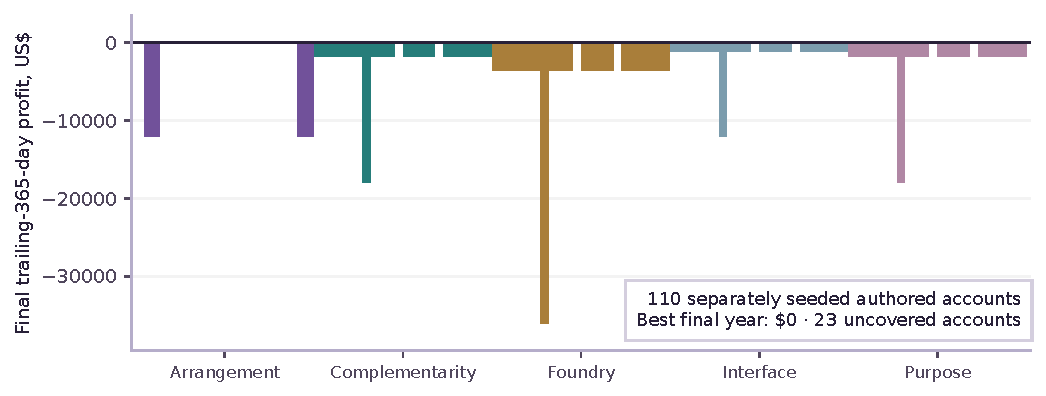
\includegraphics[width=\linewidth]{figures/financial_screen.pdf}
\caption{All 110 reported final trailing-year profits, grouped by route and sorted by case identifier. Each bar is a separate authored account. Zero is the best result; losses and uncovered obligations remain. The series neither demonstrates a scale path nor proves global impossibility.}\label{fig:finance}
\end{figure}

\subsection{Audit the opportunity set before interpreting a milestone}
Each market has eight authored buyers, at most three purchase opportunities each, and a maximum posted price of US\$40,000. Thus its loose three-year gross-contract ceiling is $8\times3\times40{,}000=\$960{,}000$ per account. No policy within that fixed market can generate a US\$3 billion annual profit from those contracts. Adding hypothetical opening equity leaves those buyer opportunities unchanged. This proves a limitation of that experiment's opportunity set, not a limitation of autonomous enterprise in general.

Some computational packages collect simulated orders, yet final-year maintenance and support can remain after finite selling opportunities end. A high cumulative collection count, a short profitable cohort or cash close to a large opening balance is not the fixed-endpoint profit target. Central purpose and arrangement refusal cases also show that non-entry can preserve capital more effectively than financing a weak offer. These observations are conditional on the registered worlds.

For every compact final case the report checks
\begin{align}
\Pi &= R-E,\\
C &= C_0+\Pi+L,\\
C_{\rm protected}&=C-C_{\rm available},
\end{align}
with exact integer microUSD, opening equity $C_0$, company profit $\Pi$, revenue $R$, incurred expenses $E$, final cash $C$, and unpaid obligations $L$ in the final no-custody summaries. The $+L$ term explains why cash can remain after an incurred expense has not been paid. These identities do not validate demand, cost calibration, tax law or a business. Earlier live states with custody/other flows require the full native equation rather than this terminal-summary identity.

The report checks all 110 summary rows and their original window labels; it does not claim to replay the omitted 94 raw histories in the compact public export. The original verdict discloses that some final independent-validator code was executed by the integration owner. Source agreement and procedural separation remain different from external certification. Unknown lost-process resources, upstream human attention and actual bills remain unknown.

\section{From an instrument to an expanding productive arrangement}
The object to construct is the complete arrangement: beneficiary outcome, missing means, production, acceptance, voluntary participation, rights, financing and recovery \cite{economy,frontier}. An exact model result can reveal a missing condition with considerable future value. Capturing that value requires additional facts: a qualified use, a willing buyer, a complete competitive offer, supplied capacity, positive full-cost surplus and timely spendable resources.

\subsection{Choose capital jointly with the productive method}
Prospective starting capital is a decision variable. US\$100,000 remains a reference and a historical condition, not a universal seed requirement. US\$1 billion is an eligible financing hypothesis where its costs, terms and availability are modeled, not received cash or a ceiling. New work should compare non-entry, staging and appropriately smaller/larger capital with complete opportunity, interest, dilution/control and downside terms. Preserve old cohorts rather than retrospectively top them up.

A necessary resource inequality for a new commitment at time $t$ is
\begin{equation}
\text{available cash}_t\ \geq\ \text{permitted immediate commitment}_t,
\end{equation}
after protected obligations and the native reservation semantics are applied. Expected profit, a financing promise and an accepted-but-uncollected invoice do not satisfy it. A reservation is not automatically an expense, and releasing collateral is not income. The native \texttt{JournalAccount} and adaptive \texttt{Account} remain the financial authority; this report opens no alternative ledger or business account.

\subsection{Productivity, surplus and profit capture need different comparisons}
The primary productivity benchmark is competent frontier AI/agents versus competent 100\% human workers using conventional software, under the same outcome, acceptance, rights, deadlines and support obligations. Genuine conventional software automation stays at machine speed. The AI arm must count actual or explicitly modeled internal human work; any nonzero such work is a hybrid case rather than strict 100\% autonomy. Buyer consent is a different participation burden. None of the reviewed finite algorithm comparisons supplies a measured full human lifecycle benchmark.

Competitive AI vendors, self-service, buying an existing instrument and not purchasing are additional complete commercial alternatives. They can restrict the share of productivity gains a company retains. A human-wage comparison alone does not establish a sustainable price when an equally capable rival can supply the same result cheaply. A conventional algorithmic tie alone does not disprove viable commerce when complete delivery still solves a paid problem. Both comparisons belong in a credible operating experiment.

For annual complete-cost profit target $G$, a homogeneous accounting model with contribution $m>0$ per collected accepted contract and annual fixed expense $F$ requires at least $\lceil(G+F)/m\rceil$ contracts. That is arithmetic necessity, not a demand forecast. Dated acquisition, capacity, acceptance, collection, lockup and support must support the schedule; correlated failure can invalidate an attractive average. The operational075 worksheet exposes these missing conditions rather than establishing them.

\subsection{Retain generative means, not a fixed ceremony}
Keep the callable instrument, its executable certificate, the assumptions that make it applicable and the concise lesson about failed use. A successor may compose complementary means or invent a missing connector. Composition is causal only when the interface and effects actually make the next operation feasible; a list of module names is insufficient. Removing a component, giving equal content to an ordinary method, and allowing that method to construct its own complete route are decision-relevant controls.

An improving discovery procedure needs a more demanding test: freeze a proposal/selection/experiment policy, compare it with both its predecessor and a strong conventional improver from matched starting means, then evaluate fresh complete campaigns with acquisition, checking, failed search and maintenance charged. A new artifact, a better-equipped successor and an improved inventor remain three different results. The current report establishes no persistent recursive improvement of discovery.

\section{The long-horizon program and the next decisive work}
The long-horizon ambition is an invention-and-production infrastructure that can expand useful scientific measurement, qualified manufacturing and energy capability. Knowledge can support new instruments; instruments can make new experiments feasible; accepted discoveries can support productive methods; valid collected surplus or justified financing can fund installed capacity. Physical output, useful energy, economic surplus and company profit are separate quantities. None grows merely because an artifact count grows.

The reviewed studies supply intermediate methods and sharp boundaries, not that eventual infrastructure. They show why the route must be mechanistic: acquire the observation that distinguishes the required alternatives; build the interface that exposes the useful invariant; combine production means under the full resource contract; establish acceptance; design a complete voluntary offer; pay for continuation from resources actually available. These steps make the ambition testable without treating a desired scale as an observed result.

\begin{table}[htbp]\centering\small
\begin{tabularx}{\linewidth}{@{}P{2.55cm}YY@{}}\toprule
Dependency & Next decisive construction or evidence & Stop or revise when\\\midrule
Local manufacturing decision & Same-specimen independent local truth, calibrated absolute reference, known spatial kernels and adequate directions; freeze the actual release target & Available observations still leave incompatible accepted/rejected worlds\\
Optical access instrument & Realizable calibrated coupled reflector or a separately justified invariant purpose with independent reference objects & Hardware/access/dispersion burden erases the qualified advantage\\
Water delivery qualification & Authoritative channel, metrology, time and batch-release bindings; freeze fresh dates only after the proxy is justified & Qualified volume remains unsupported; do not replace missing values with favorable assumptions\\
Discovery allocation & Fresh independent panel, purpose-specific errors and matched total acquisition/reference/assay costs; permit simpler complete routes & The ordinary method meets the same outcome more cheaply, or prospective physical service remains unqualified\\
Complete commercial continuation & Source-grounded voluntary demand, dated capacity, accepted artifacts, costs, remedy obligations and valid cash; native full-window observation & Buyer outside options, liquidity or complete costs defeat the proposed offer\\\bottomrule
\end{tabularx}
\caption{Proposed work, not completed new experiments. These are selected dependencies; an unrelated stronger consequential arrangement remains eligible. Supporting paper/checker work must lead back to a discriminating construction or delivery.}\label{tab:next}
\end{table}

A candidate may be retired while its useful instrument remains. Another candidate can be chosen when it offers a sharper route to a consequential outcome. The mission need not remain water, optics or one historical task catalogue. It also need not invent a new mathematical primitive at every step. Established mechanisms are welcome when they change what can actually be delivered. Expansion should follow accepted evidence, useful variety and complete economics rather than the preservation of a preferred story.

\insight{\centering\textbf{Construct the means. Establish the consequence.}\par
\textbf{Deliver useful work. Finance the next warranted step.}\par\smallskip
FIND YOUR ALPHA. BUILD YOUR SUCCESSOR $\Omega$.}

\section{Conclusion}
The experiments make the flywheel more concrete and more selective. Executable programs can call earlier programs; exchanged acquisition can remove fixed nuisance gains; uncertainty sets can support a purpose without full reconstruction; complementary processes can satisfy duties that components miss. Controls also show when ordinary methods tie, a measured interface fails, an analogy does not transfer or an economic screen cannot represent the desired scale.

The next substantive achievement is a connected, accepted productive arrangement whose enabling construction changes a distinct successor's complete technical or economic possibilities under fair alternatives. Further progress would show that the discovery process itself improves on fresh campaigns. Very large sustained profit, industry creation and physical expansion require additional operating evidence. The report provides the artifacts, distinctions and next decisions needed to pursue those outcomes while preserving the useful baseline.

\textbf{Research status.} AI-assisted source review, original synthesis, deterministic local reproduction and compact data checking. Existing studies include human-authored models, included-agent constructions and procedurally separated checks; their model and labor scopes remain distinct. No paid model API, new paid service, real transaction, outreach, device actuation or native financial mutation was used for this report. This is a research publication, not a claim of external peer review, achieved AGI/ASI or an enterprise-runtime release.

\clearpage\appendix
\section{Exact sources and study boundaries}
The complete machine-readable map is \texttt{evidence/sources.json}. Every entry includes the original public repository path, full commit, Git blob identity, SHA-256 and permalink. The compact numeric extraction is \texttt{evidence/observations.json}. Its source hashes identify the reviewed bytes; this is not remote attestation or a substitute for the underlying artifacts.

\begin{longtable}{@{}P{2.8cm}P{4.1cm}P{7.4cm}@{}}\toprule
Study & Reviewed revision & Boundary retained\\\midrule\endhead
Main report baseline & \nolinkurl{215b22a5ed73b82ac1d909328d60157c48bd9958} & Published main sources, including the earlier flywheel editions and completed public portfolio; later branch studies are separate.\\
Published foundry & Same main; protocol \nolinkurl{fa7a1117b91340afb27288ec09adbc33926d9ba4} & Protocol public before substantive execution; 144 crossed records, 30 accepted and six nonidentifiable requests per arm.\\
Public portfolio R2 & Same main; original integrated source \nolinkurl{e67aa09031583f976a39c8406ae86585b02cde76} & 110 native authored cases; compact summaries and original independent-review limits, not 110 new full replays.\\
Next-series N1/N3 & Same main; results originally \nolinkurl{00946cf112e457eabf0e5aa8163e931cb562cf54} & Model instruments and missing provenance; zero fresh water dates/raw NIST rows in that stage.\\
Paired acquisition & Same main; scientific freeze \nolinkurl{e30b8af4f6ff9b06d6676c76f53d90d6d65e0dda} & Exact source checked around reproduction; conventional ties and four undetected-error witnesses retained.\\
Optical / WATER-01 & \nolinkurl{a5df603854f98cbd673204258c8d768e0c759975} & PR152 source slice; model optics and seven historical water dates. Open-branch evidence is not a published runtime.\\
Portfolio071 & \nolinkurl{418440e4587165488ccbf5a9d6bc04ba375a4675} & PR151 is separate from PR153; original finite science and incomplete 24-arm reconciliation are preserved.\\
NEXT072 & \nolinkurl{b2d41c513dfc950648b39e64627a77ada0137a22} & Public measured-panel replay, exposed controls, no new assays or accepted K2 physical service.\\
Outlearning073 & \nolinkurl{21f78996d25fe1d17b2c560be07e715ac8dc48d9} & Seven native hypothetical scenarios; source/freeze and independent verdict retain their own identities.\\
Other outlearning & \nolinkurl{7f94f8fed2026b14b53f4ff7c94e1a1f3c35ae68} & Separate PR161, 18 accounts and original freeze; no pooled verdict.\\
Grid074 & \nolinkurl{000d2b30f2073a228c286c5ae736af71ab6fec41} & Development falsification, no completed ordinary comparator or blinded confirmation.\\
Operational075 & \nolinkurl{b32d6913754a6b83c3df76604647418de70d9748} & Actual original computational-client acceptance; scale worksheet remains conditional, with no native account.\\\bottomrule
\end{longtable}

The source review separates report date from later source status. Main contains some integrated studies and preserved research editions. Other records are on explicitly pinned open branches. A public result file, green dedicated workflow, merged source, released artifact and accepted operation of the downloaded release remain different facts. This paper's publication does not promote any of those studies into a production enterprise.

\section{Reproduce the report}
From the report directory, Python 3.11 or later suffices for its compact auditor and exact rational illustration:
\begin{lstlisting}
python audit.py --output /absolute/new/report-audit.json
python -m unittest discover -s . -p 'test_*.py' -v
\end{lstlisting}
The auditor checks all 110 compact case identities and specified terminal money identities, the 36-request foundry denominators, the conventional win, the paired contract counts, outlearning's tied acceptance and diagnostic cost, and retained scope flags. It is deliberately smaller than a native account verifier. Seven regression/mutation tests check missing cases, losses replaced with zero, equity turned into profit, erased unpaid obligations, a hidden conventional win and the exact information witness. The public snapshot contains no signing authority.

The two comparison figures are generated from the compact observations. Matplotlib is required only to regenerate their vector PDFs; final figures and their exact CSV values are included:
\begin{lstlisting}
python make_figures.py
make
make check
python verify.py
python package.py --output /absolute/new/report-publication
\end{lstlisting}
The source is suitable for a standard pdfLaTeX/BibTeX installation or a LaTeX editor. \texttt{paper.tex} is the main file. Public citation metadata, editable source, bibliography, figure sources, audit, result snapshot and checksums accompany the PDF. The report does not require model/provider keys, a wallet or paid service.

\subsection{The reproduced original procedures}
From a checkout at the report baseline, use new output paths and the repository's pinned numerical environment:
\begin{lstlisting}
python docs/agi-alpha-flywheel/examples/check_foundry.py
python experiments/next_series_20261102_365c3d6c/verification/verify_n1.py --output /absolute/new/n1.json
python experiments/next_series_20261102_365c3d6c/verification/verify_n3.py --output /absolute/new/n3.json
OPENBLAS_NUM_THREADS=1 OMP_NUM_THREADS=1 python -m experiments.paired_acquisition_20261102.run --output /absolute/new/paired --expected-freeze-sha256 db80989740105baeca37be68b7fa9615c436965ea9ea160712f258ca3da490dc --source-commit 215b22a5ed73b82ac1d909328d60157c48bd9958 --execution-label report-engineering-reproduction
\end{lstlisting}
The numerical environment used for this report is Python 3.12.14, NumPy 2.3.5 and SciPy 1.17.0. These repeated exposed cases are engineering reproductions rather than new confirmation samples. The report's verification receipt records their commands, source hashes and accepted scope. It does not claim that another reviewer or physical laboratory independently repeated this report.

\texttt{prepare\_evidence.py} recreates the compact extraction from the exact public commits. It requires a Git checkout containing those commits and may materialize public blobs. It neither opens a native financial account nor reads private account directories. A source ZIP supports offline audit of the frozen compact snapshot; fetching original study sources is separately necessary to repeat their full procedures. The old artifacts remain unchanged.

\section{Later development: Enterprise078, 3 November}
The separately reviewed Enterprise078 checkpoint \cite{enterprise078} records source-qualification and whole-buyer-choice repairs after the main research period. A supplied candidate tree could previously be signed without matching the acceptance modules actually loaded; a source-bound counterexample exposed that gap and prompted a fail-before-preparation repair. An additional counterexample showed that two substitute outputs can each satisfy individual value/budget checks while their joint offer loses to a conventional service. Shared wallet accounting alone is insufficient to establish joint voluntary utility.

At reviewed head \nolinkurl{7586d3edf8e8837f1075ecc5afdb6369af77ce76}, the native catalog activation remains unimplemented. Exact SQL/CSV artifacts, an inactive signed proposal and local tests do not grant native admission, authorize a sale or establish commercial profit. Historical modeled profit of US\$19,574.55 excludes newly unresolved construction/model/host attribution; updated complete-cost profit is unknown. These later corrections are useful engineering learning, not another positive outcome inserted into the 2 November experiments. No source or financial history is changed by this report.

\section{Publication and practical handoff}
The report is an additive publication with a distinct filename and report release identity. Earlier AGI ALPHA FLYWHEEL editions 1.0 and 1.1, OUT-ACCELERATE and all original study paths remain unchanged. The repository entry point links the PDF, source directory and evidence. A narrow publication workflow compiles the report, runs the compact audit and its controls, verifies source/PDF identities and packages versioned assets. Normal repository checks and review remain applicable. No paid runner, new service, account access or permission change is required by this publication.

The immediate handoff is small: select one consequential complete arrangement; identify the missing means and the strongest complete alternative; construct the discriminating test; freeze the acceptance and full-resource comparison before observing the new outcome; retain the useful artifact and concise applicability lesson; then decide whether a valid commercial offer or another construction is justified. The next observation or delivery should change a decision. A paper, checker or larger simulation is supporting work and must not become the substitute mission.

\bibliographystyle{unsrtnat}\bibliography{references}
\end{document}
